% Word Embeddings: 2D scatter-plot visualisation for teaching
% Compile with:
%   pdflatex similar_words.tex
%   convert -density 200 similar_words.pdf -quality 95 similar_words.png

\documentclass[tikz,border=10pt]{standalone}
\usepackage{tikz}
\usetikzlibrary{arrows.meta}

% --- Cluster colours ---
\definecolor{animalcol}   {RGB}{0,140,130}    % teal
\definecolor{royaltycol}  {RGB}{210,100,0}    % orange
\definecolor{foodcol}     {RGB}{150,40,160}   % purple
\definecolor{transportcol}{RGB}{30,100,180}   % blue
\definecolor{emotioncol}  {RGB}{190,40,70}    % crimson

\begin{document}
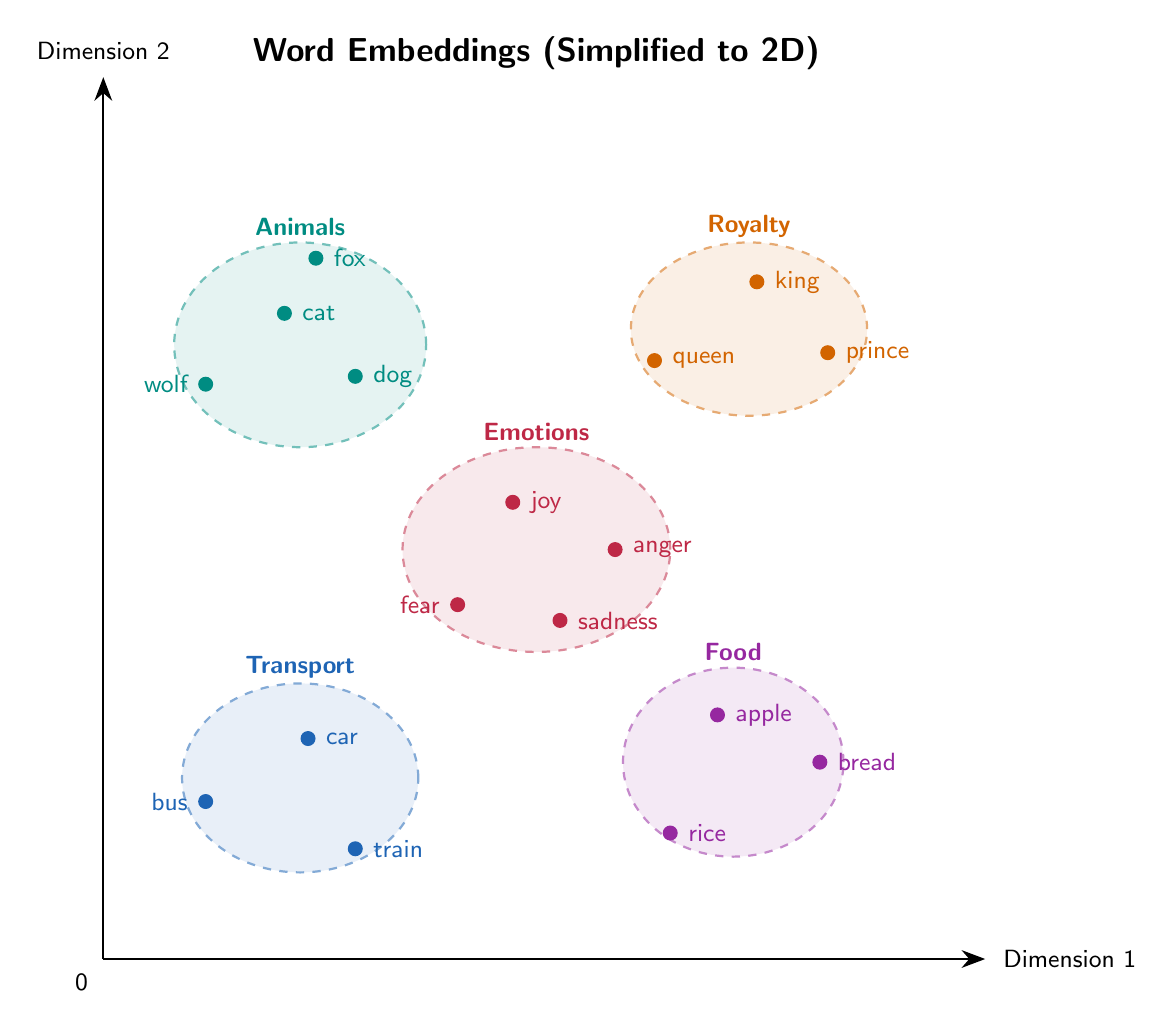
\begin{tikzpicture}[font=\sffamily]

% Title
\node[font=\large\bfseries\sffamily] at (5.5,11.5)
    {Word Embeddings (Simplified to 2D)};

% Axes — origin at bottom-left, positive quadrant only
\draw[-{Stealth[length=3mm]}, thick] (0,0) -- (11.2,0);
\node[font=\small\sffamily, right=3pt] at (11.2,0) {Dimension 1};

\draw[-{Stealth[length=3mm]}, thick] (0,0) -- (0,11.2);
\node[font=\small\sffamily, above=3pt] at (0,11.2) {Dimension 2};

% Origin marker
\node[font=\small\sffamily, below left=2pt] at (0,0) {0};

% ================================================================
% ANIMALS (teal) --- upper-left
% ================================================================
\fill[animalcol!10]  (2.5,7.8) ellipse (1.6 and 1.3);
\draw[animalcol!55, dashed, thick] (2.5,7.8) ellipse (1.6 and 1.3);
\node[font=\small\bfseries\sffamily, text=animalcol] at (2.5,9.3) {Animals};

\filldraw[animalcol] (2.3, 8.2) circle (2.5pt);
\node[font=\small\sffamily, text=animalcol, right=3pt] at (2.3, 8.2) {cat};

\filldraw[animalcol] (3.2, 7.4) circle (2.5pt);
\node[font=\small\sffamily, text=animalcol, right=3pt] at (3.2, 7.4) {dog};

\filldraw[animalcol] (1.3, 7.3) circle (2.5pt);
\node[font=\small\sffamily, text=animalcol, left=3pt]  at (1.3, 7.3) {wolf};

\filldraw[animalcol] (2.7, 8.9) circle (2.5pt);
\node[font=\small\sffamily, text=animalcol, right=3pt] at (2.7, 8.9) {fox};

% ================================================================
% ROYALTY (orange) --- upper-right
% ================================================================
\fill[royaltycol!10]  (8.2,8.0) ellipse (1.5 and 1.1);
\draw[royaltycol!55, dashed, thick] (8.2,8.0) ellipse (1.5 and 1.1);
\node[font=\small\bfseries\sffamily, text=royaltycol] at (8.2,9.3) {Royalty};

\filldraw[royaltycol] (8.3, 8.6) circle (2.5pt);
\node[font=\small\sffamily, text=royaltycol, right=3pt] at (8.3, 8.6) {king};

\filldraw[royaltycol] (7.0, 7.6) circle (2.5pt);
\node[font=\small\sffamily, text=royaltycol, right=3pt] at (7.0, 7.6) {queen};

\filldraw[royaltycol] (9.2, 7.7) circle (2.5pt);
\node[font=\small\sffamily, text=royaltycol, right=3pt] at (9.2, 7.7) {prince};

% ================================================================
% EMOTIONS (crimson) --- centre
% ================================================================
\fill[emotioncol!10]  (5.5,5.2) ellipse (1.7 and 1.3);
\draw[emotioncol!55, dashed, thick] (5.5,5.2) ellipse (1.7 and 1.3);
\node[font=\small\bfseries\sffamily, text=emotioncol] at (5.5,6.7) {Emotions};

\filldraw[emotioncol] (5.2, 5.8) circle (2.5pt);
\node[font=\small\sffamily, text=emotioncol, right=3pt] at (5.2, 5.8) {joy};

\filldraw[emotioncol] (6.5, 5.2) circle (2.5pt);
\node[font=\small\sffamily, text=emotioncol, right=3pt] at (6.5, 5.2) {anger};

\filldraw[emotioncol] (4.5, 4.5) circle (2.5pt);
\node[font=\small\sffamily, text=emotioncol, left=3pt]  at (4.5, 4.5) {fear};

\filldraw[emotioncol] (5.8, 4.3) circle (2.5pt);
\node[font=\small\sffamily, text=emotioncol, right=3pt] at (5.8, 4.3) {sadness};

% ================================================================
% FOOD (purple) --- lower-right
% ================================================================
\fill[foodcol!10]  (8.0,2.5) ellipse (1.4 and 1.2);
\draw[foodcol!55, dashed, thick] (8.0,2.5) ellipse (1.4 and 1.2);
\node[font=\small\bfseries\sffamily, text=foodcol] at (8.0,3.9) {Food};

\filldraw[foodcol] (7.8, 3.1) circle (2.5pt);
\node[font=\small\sffamily, text=foodcol, right=3pt] at (7.8, 3.1) {apple};

\filldraw[foodcol] (9.1, 2.5) circle (2.5pt);
\node[font=\small\sffamily, text=foodcol, right=3pt] at (9.1, 2.5) {bread};

\filldraw[foodcol] (7.2, 1.6) circle (2.5pt);
\node[font=\small\sffamily, text=foodcol, right=3pt] at (7.2, 1.6) {rice};

% ================================================================
% TRANSPORT (blue) --- lower-left
% ================================================================
\fill[transportcol!10]  (2.5,2.3) ellipse (1.5 and 1.2);
\draw[transportcol!55, dashed, thick] (2.5,2.3) ellipse (1.5 and 1.2);
\node[font=\small\bfseries\sffamily, text=transportcol] at (2.5,3.7) {Transport};

\filldraw[transportcol] (2.6, 2.8) circle (2.5pt);
\node[font=\small\sffamily, text=transportcol, right=3pt] at (2.6, 2.8) {car};

\filldraw[transportcol] (1.3, 2.0) circle (2.5pt);
\node[font=\small\sffamily, text=transportcol, left=3pt]  at (1.3, 2.0) {bus};

\filldraw[transportcol] (3.2, 1.4) circle (2.5pt);
\node[font=\small\sffamily, text=transportcol, right=3pt] at (3.2, 1.4) {train};

\end{tikzpicture}
\end{document}
